\section{Motorization: the mechanics}
The motorization of the telescope passes through two mechanics adjustments:
\begin{enumerate}
    \item motorize the RA movement, exploiting the native tracker mechanism;
    \item motorize the DEC movement, which natively has no gears.
\end{enumerate}

\subsection{RA motorization}
The telescope's mount has already a tracking mechanism motorized by a 3W synchronous motor.
So, in principle, it is only a matter of substitute this old motor, with a new programmable stepper motor.

The gears are composed by:
\begin{itemize}
    \item a 359 teeth stage (1 tooth for each degree, fantastic);
    \item an endless screw (worm) mounted on a shaft through a clutch.
\end{itemize}
Using this structure, for a continuous sky tracking, the elder motor would complete a round of the worm in 4 minutes.
Thus, this mechanism rotates the mount with the velocity of a degree in 4 minutes (which is the velocity of the sky moving away in the night).

We have reduced the ratio by a third adding two other gears (see figure \ref{fig:RA_mechanization}): 60 teeth gear positioned in the shaft and a 20 teeth gear on the motor shaft.
\\
\begin{minipage}{.4\textwidth}
    \begin{tabular}{cc|c}
        ratio gear 1 & ratio gear 2 & total ratio \\
        \hline
        1/360 & 1/3 & 1/1080 \\
        \hline
    \end{tabular}
    \captionof{table}{Total reduction of RA mechanization.}
    \label{tab:RA_mechanization}
\end{minipage}
\\
\begin{minipage}{.4\textwidth}
    \centering
    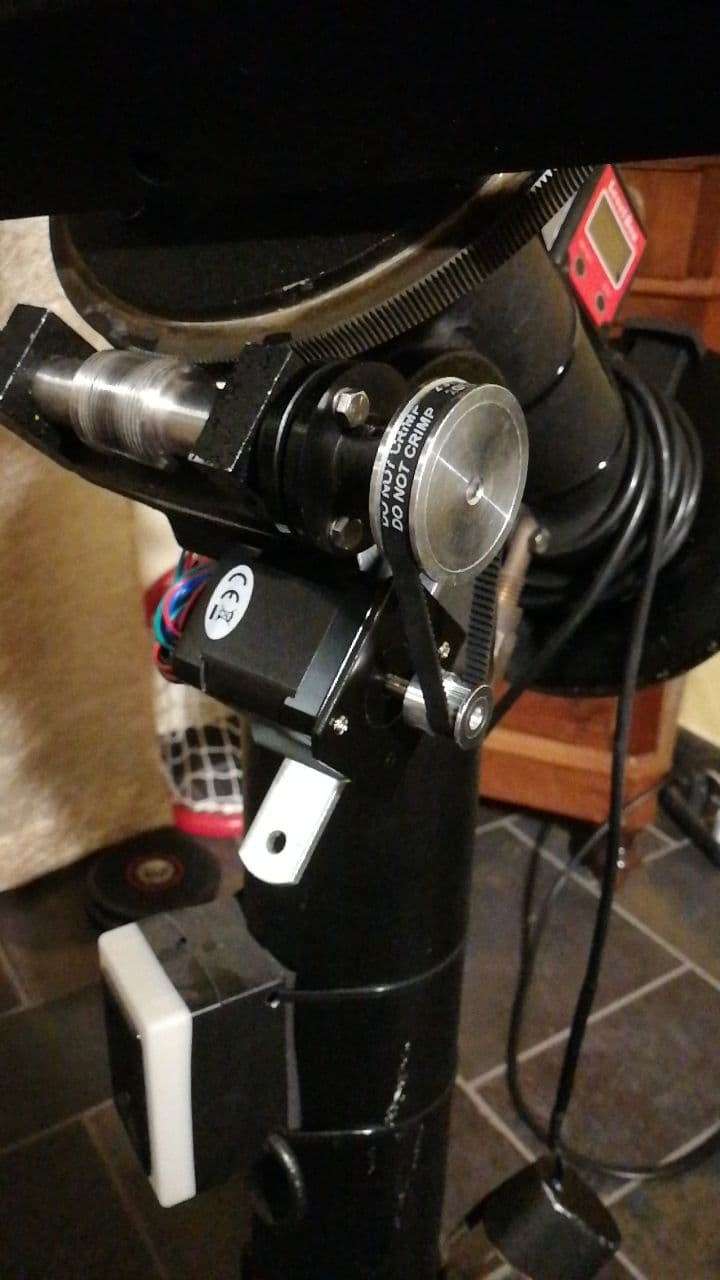
\includegraphics[scale=0.6]{RA_motorization.jpg}  
    \captionof{figure}{Nema 17 stepper motor and gear adjustment.}
    \label{fig:RA_mechanization}         
\end{minipage}
\\
We have choose to install a nema 17 stepper motor with the specifics in table \ref{tab:nema_17_specifics}

\subsection{DEC motorization}
The mechanization of the DEC axis was a bit more complicated since there was not a built-in gear to use.
We tried different versions.
A first successfully try was to exploit a stand-alone disk.
On the edge of the latter are present some ticks and grades: it was used a declination angle teller.

As told above, we have tried different configurations but same stepper motor is used.

\subsubsection{DEC V1}
The first version is made using the built-in graded disk mounted on the telescope.
On this, is attached a 32cm long chain strip.
Then, a 1/3 reduction shaft is positioned between the first gear and the stepper motor's gear.
The total reduction with all gear specifics is reported in table \ref{tab:DEC_gear_spec}.
Figure \ref{fig:DEC_mechanism} is a picture of the mechanism.

\begin{minipage}
    {0.5\textwidth}
    \centering
    \textbf{DEC-V1 stages}\\
    \begin{tabular}{ccccc}
        \hline
        Gear number & 1 & 2 & 3 & 4 \\
        number of teeth & 188 & 20 & 60 & 20 \\
        \hline
        total ratio & \(\sim \frac{1}{28}\) &&&
    \end{tabular}
    \captionof{table}{DEC mechanism's gear specifics.}
    \label{tab:DEC_gear_spec}
\end{minipage}
\\
\begin{minipage}
    {0.5\textwidth}
    \centering
    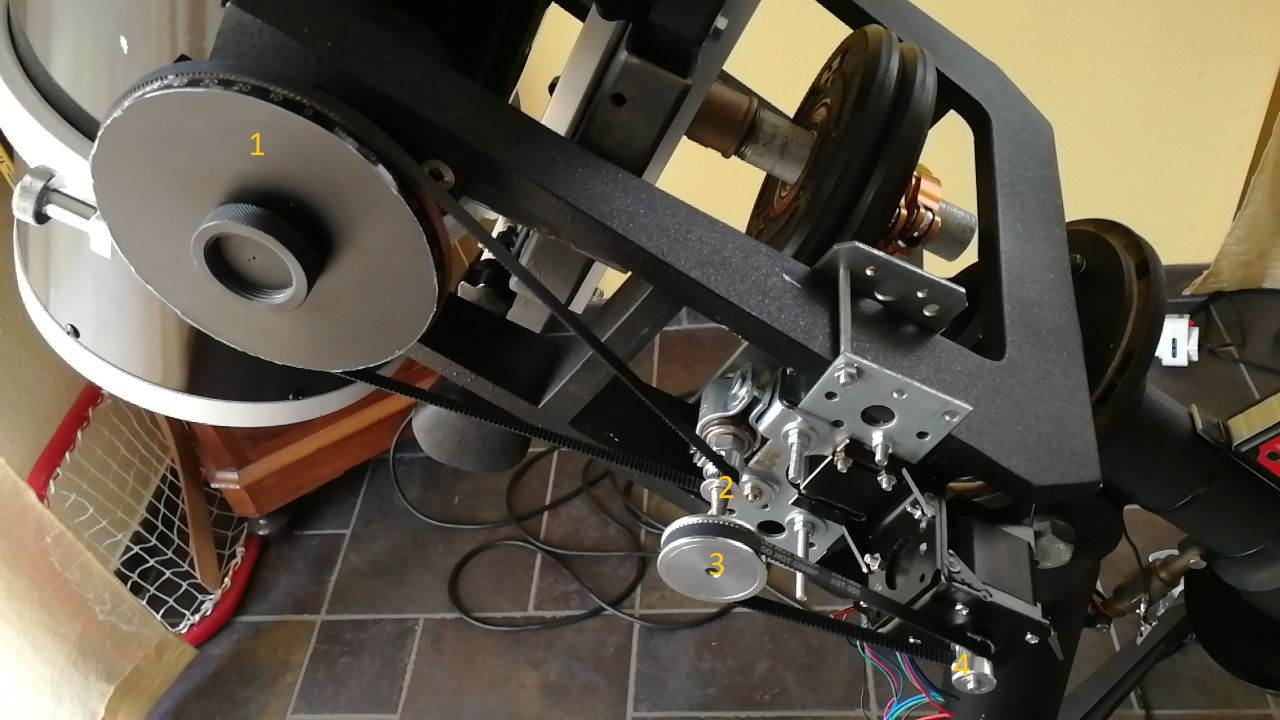
\includegraphics[scale=.28]{DEC_motorization.jpg}
    \captionof{figure}{DEC mechanism.}
    \label{fig:DEC_mechanism}
\end{minipage}
\\
This solution seemed to be efficient, but easy to adjust.
Also, the stage reduction is too low for a good movement precision.

\subsubsection{DEC V2}
The second version made uses again the built-in graded disk mounted on the telescope.
Also on this construction is glued a 32cm long chain strip.
Then, a 1/9 reduction is positioned between the first stage and the stepper motor.
The total reduction with all gear specifics is reported in table \ref{tab:DEC_gear_spec_v2}.
Figure \ref{fig:DEC_mechanism_v2} is a picture of the mechanism.

\begin{minipage}
    {0.5\textwidth}
    \centering
    \textbf{DEC-V2 stages}\\
    \begin{tabular}{ccccccc}
        \hline
        Gear number & 1 & 2 & 3 & 4 & 5 & 6\\
        number of teeth & 188 & 20 & 60 & 20 & 60 & 20\\
        \hline
        total ratio & \(\sim \frac{1}{84}\) &&&
    \end{tabular}
    \captionof{table}{DEC mechanism's gear specifics.}
    \label{tab:DEC_gear_spec_v2}
\end{minipage}
\\
\begin{minipage}
    {0.5\textwidth}
    \centering
    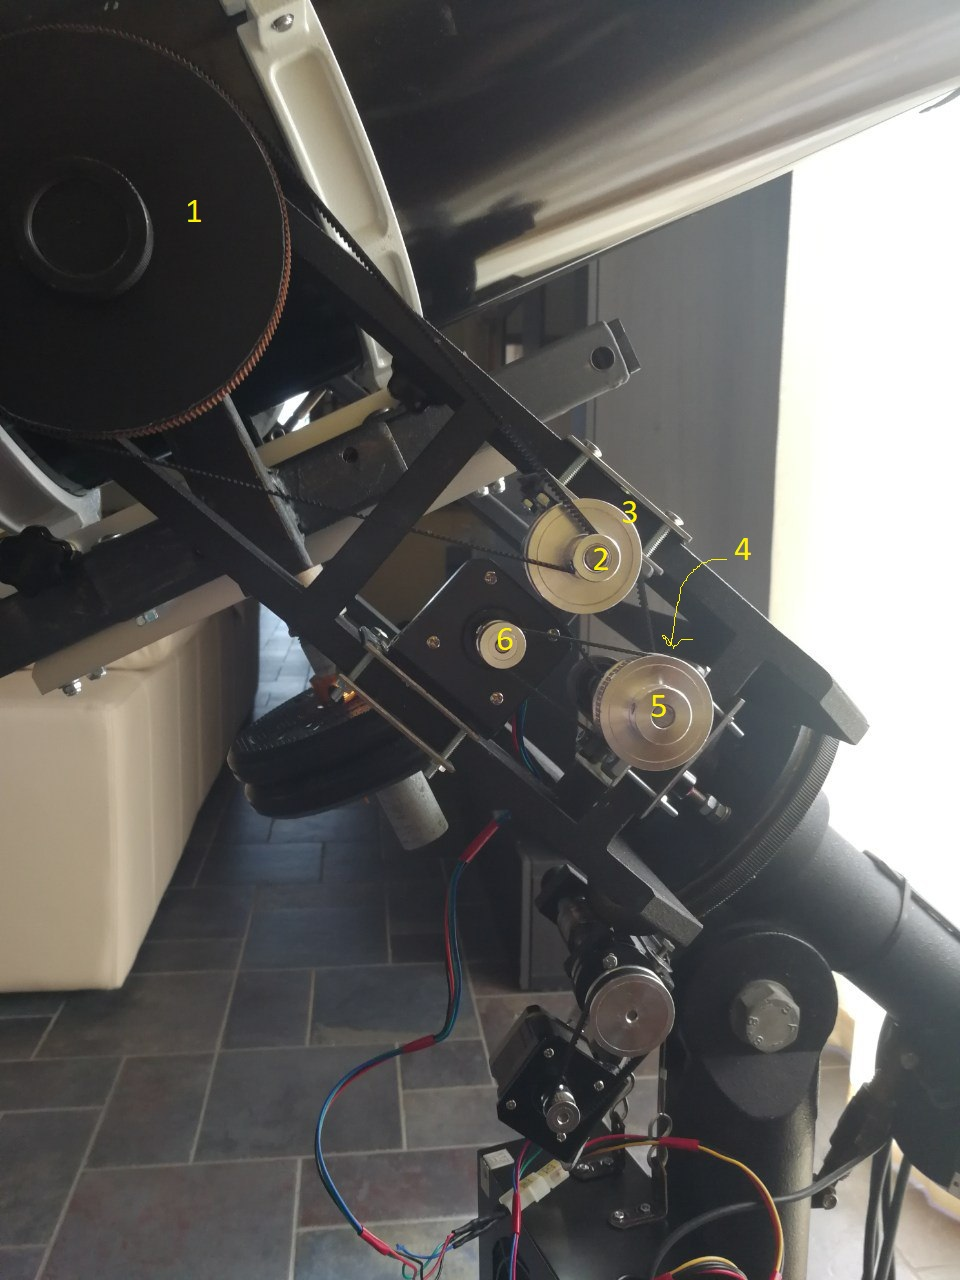
\includegraphics[scale=.2]{DEC_v2.jpg}
    \captionof{figure}{DEC V2 mechanism.}
    \label{fig:DEC_mechanism_v2}
\end{minipage}

\subsection{DEC V3}
The third version uses a 3D printed double-belt gear mounted on the telescope.
Then, a 1/10 ratio is obtained using a worm gear and another 1/3 is obtained between the worm and the final gear.
The total reduction with all gear specifics is reported in table \ref{tab:DEC_gear_spec_v3}.
Figure \ref{fig:DEC_mechanism_v3} is a picture of the mechanism.

\begin{minipage}
    {0.5\textwidth}
    \centering
    \textbf{DEC-V2 stages}\\
    \begin{tabular}{cccccc}
        \hline
        Gear number & 1 & 2 & 3 & 4 & worm\\
        number of teeth & 180 & 30 & 60 & 20 & 10\\
        \hline
        total ratio & \(\sim \frac{1}{180}\) &&&
    \end{tabular}
    \captionof{table}{DEC mechanism's gear specifics.}
    \label{tab:DEC_gear_spec_v2}
\end{minipage}
\\
\begin{minipage}
    {0.5\textwidth}
    \centering
    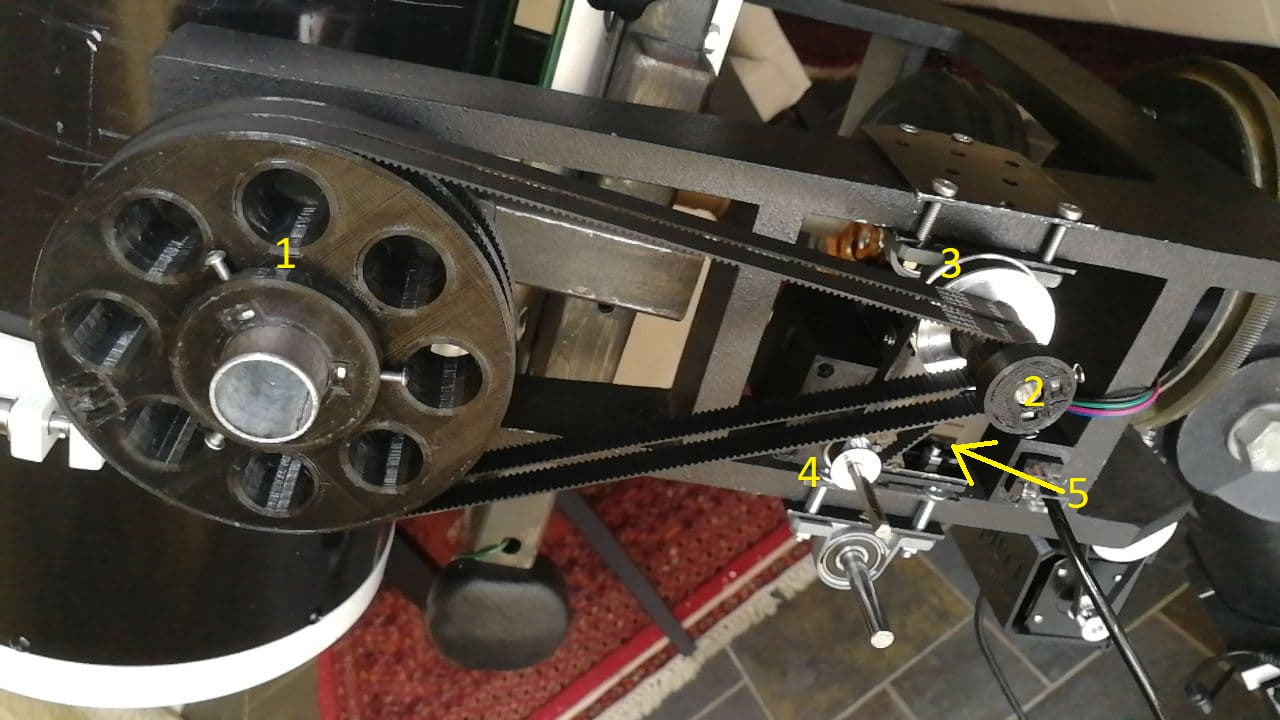
\includegraphics[scale=.6]{DEC-v3.jpg}
    \captionof{figure}{DEC V3 mechanism.}
    \label{fig:DEC_mechanism_v3}
\end{minipage}

\subsection{Focuser motorization}
Another improvement is the motorization of the focuser.
Using a nema 11 stepper motor, we have created the motor supports and the gears using a 3D printer.
The reduction stage is 3, see figure \ref{fig:focuser-box}.